% =====================================================================
%  Optimization Methods -- Seminar 01
%  HSE University, Faculty of Computer Science
%  Compile: ./build.sh  (xelatex)
% =====================================================================
\documentclass[aspectratio=169,11pt]{beamer}

\usepackage{iftex}
\ifPDFTeX
  \usepackage[T1]{fontenc}
  \usepackage[utf8]{inputenc}
  \usepackage{lmodern}
\else
  % XeLaTeX: CM Unicode, the Unicode version of Computer Modern (same look as
  % lmodern, full Cyrillic). Math stays on the classic CM fonts (no unicode-math).
  % No \defaultfontfeatures{Ligatures=TeX}: fontspec already applies it to rm/sf,
  % and on tt it would turn " into a curly quote inside code listings.
  \usepackage{fontspec}
  \setmainfont{cmunrm.otf}[
    BoldFont       = cmunbx.otf,
    ItalicFont     = cmunti.otf,
    BoldItalicFont = cmunbi.otf]
  \setsansfont{cmunss.otf}[
    BoldFont       = cmunsx.otf,
    ItalicFont     = cmunsi.otf,
    BoldItalicFont = cmunso.otf]
  \setmonofont{cmuntt.otf}[
    BoldFont       = cmuntb.otf,
    ItalicFont     = cmunit.otf,
    BoldItalicFont = cmuntx.otf]
\fi
\usepackage{amsmath,amssymb}
\usepackage{booktabs}
\usepackage{array}
\usepackage{tikz}
\usepackage{listings}

% ----------------------------- identity -----------------------------
\newcommand{\presenter}{Evgeny Baulin}
\newcommand{\contact}{Telegram: @tarakan\_tuc}
\newcommand{\seminardate}{Seminar 01}

% ----------------------------- look ---------------------------------
\definecolor{hseblue}{RGB}{16,45,105}
\definecolor{hseaccent}{RGB}{198,40,40}
\definecolor{hsegray}{RGB}{108,114,126}
\definecolor{hselight}{RGB}{235,239,246}

\usetheme{default}
\setbeamertemplate{navigation symbols}{}
\setbeamercolor{structure}{fg=hseblue}
\setbeamercolor{frametitle}{fg=hseblue}
\setbeamercolor{framesubtitle}{fg=hsegray}
\setbeamerfont{frametitle}{size=\large,series=\bfseries}
\setbeamerfont{framesubtitle}{size=\small,series=\mdseries}
\setbeamertemplate{frametitle}{%
  \vspace{0.55em}%
  \begin{beamercolorbox}[wd=\paperwidth,leftskip=0.9em,rightskip=0.9em]{frametitle}%
    \insertframetitle\par
    {\usebeamerfont{framesubtitle}\usebeamercolor[fg]{framesubtitle}\insertframesubtitle\par}%
    \vspace{0.15em}{\color{hseaccent}\rule{2.2em}{1.6pt}}%
  \end{beamercolorbox}%
}
\setbeamertemplate{footline}{%
  \hbox{\begin{beamercolorbox}[wd=\paperwidth,ht=2.2ex,dp=1.4ex,leftskip=0.9em,rightskip=0.9em]{}%
    {\color{hsegray}\scriptsize HSE UNIVERSITY \quad\textbar\quad OPTIMIZATION METHODS
     \textperiodcentered\ SEMINAR 01 \hfill \insertframenumber}%
  \end{beamercolorbox}}%
}
\setbeamertemplate{itemize item}{\color{hseaccent}\textbullet}
\setbeamertemplate{itemize subitem}{\color{hsegray}--}

% kicker label + takeaway strip
\newcommand{\kicker}[1]{{\color{hseaccent}\scriptsize\bfseries\MakeUppercase{#1}}}
\newcommand{\takeaway}[2]{%
  \par\smallskip\noindent
  \colorbox{hselight}{\parbox{\dimexpr\textwidth-2\fboxsep}{%
    \kicker{#1}\par\vspace{0.12em}\footnotesize #2}}\par}
\newcommand{\num}[1]{{\color{hseaccent}\bfseries #1}}

\lstset{
  language=Python, basicstyle=\ttfamily\scriptsize, keywordstyle=\color{hseblue}\bfseries,
  commentstyle=\color{hsegray}\itshape, stringstyle=\color{hseaccent},
  showstringspaces=false, columns=fullflexible, breaklines=true, frame=leftline,
  framesep=6pt, rulecolor=\color{hselight}, xleftmargin=8pt
}

\title{Optimization Methods}
\subtitle{Seminar 01 \textperiodcentered\ Basic concepts: gradients, Hessians, optimality conditions}
\author{\presenter}
\institute{HSE University, Faculty of Computer Science}
\date{2025--2026}

\begin{document}

% ===================================================================
\begin{frame}[plain]
  \vspace{1.2em}
  {\color{hsegray}\scriptsize HSE UNIVERSITY \quad\textbar\quad OPTIMIZATION METHODS
    \textperiodcentered\ SEMINAR 01}\\[1.6em]
  {\color{hseblue}\Huge\bfseries Optimization Methods}\\[0.5em]
  {\color{hseblue}\Large Basic concepts of optimization}\\[0.4em]
  {\color{hsegray}\large Minima, gradients, Hessians, convexity, feasible directions}\\[1.4em]
  {\color{hseaccent}\rule{4em}{2pt}}\\[1.2em]
  {\small \presenter \quad\textbar\quad \contact \quad\textbar\quad \seminardate}
\end{frame}

% ===================================================================
\begin{frame}{Today we build the vocabulary of the whole course}
  {Everything we do later --- gradient descent, Newton, constrained problems --- is written in these five words.}
  \vspace{0.4em}
  \begin{columns}[T,onlytextwidth]
    \begin{column}{0.48\textwidth}
      \kicker{seminar goals}\\[0.5em]
      \num{1}\ \textbf{Define} \hfill\\ {\small local vs.\ global minimum, stationary point}\\[0.45em]
      \num{2}\ \textbf{Compute} \hfill\\ {\small gradients and Hessians without mistakes}\\[0.45em]
      \num{3}\ \textbf{Classify} \hfill\\ {\small stationary points: min, max, saddle}
    \end{column}
    \begin{column}{0.48\textwidth}
      \vspace{2.05em}
      \num{4}\ \textbf{Recognise} \hfill\\ {\small convex sets and convex functions}\\[0.45em]
      \num{5}\ \textbf{Handle boundaries} \hfill\\ {\small feasible directions and the inequality form of optimality}
    \end{column}
  \end{columns}
  \vspace{0.5em}
  \takeaway{takeaway}{A stationary point is a \emph{candidate}, not an answer. Most of today is about telling
    candidates apart.}
\end{frame}

% ===================================================================
\begin{frame}{The problem set for today}{Eleven exercises in four blocks. Each one gets its own slide, and then its solution gets another.}
  \vspace{0.2em}
  \begin{columns}[T,onlytextwidth]
    \begin{column}{0.49\textwidth}
      \kicker{block 1 \textperiodcentered\ gradients and Hessians}\\[0.3em]
      {\small
        \num{1}\ $f=x_1^{2}+x_2^{2}-x_1x_2$: find $\nabla f$ and $H$\\[0.2em]
        \num{2}\ $f=3x_1^{3}+2x_1x_2^{2}+4x_2^{2}$ at $(2,-1)$\\[0.2em]
        \num{3}\ $f=x_1^{2}+2x_2^{2}+3x_3^{2}+2x_1x_2-x_2x_3$}
      \vspace{0.7em}

      \kicker{block 2 \textperiodcentered\ classifying stationary points}\\[0.3em]
      {\small
        \num{4}\ $f=x_1^{2}+x_2^{2}$\\[0.2em]
        \num{5}\ $f=x_1^{2}-x_2^{2}$\\[0.2em]
        \num{6}\ $f=x_1^{3}-3x_1x_2^{2}$ (monkey saddle)\\[0.2em]
        \num{7}\ $f=x_1^{4}+x_2^{4}$}
    \end{column}
    \begin{column}{0.49\textwidth}
      \kicker{block 3 \textperiodcentered\ convexity}\\[0.3em]
      {\small
        \num{8}\ Is the disk $x_1^{2}+x_2^{2}\le4$ convex?\\[0.2em]
        \num{9}\ Is $f=x_1^{2}+x_2^{2}-4x_1x_2$ convex on $\mathbb{R}^2$?}
      \vspace{0.7em}

      \kicker{block 4 \textperiodcentered\ feasible directions}\\[0.3em]
      {\small
        \num{10}\ $\Omega=\{x_1\ge0,\ x_2\ge0\}$ at the point $(0,2)$\\[0.2em]
        \num{11}\ Directional derivative, two ways}
      \vspace{0.7em}

      \kicker{how we work}\\[0.3em]
      {\small Three minutes on your own, in pairs if you prefer. Then we solve it together on the board.
        Interrupt me during the derivation --- a question asked in the middle is worth far more than the same
        question afterwards.}
    \end{column}
  \end{columns}
\end{frame}

% ===================================================================
\begin{frame}{Warm-up: read the picture before you differentiate}
  {Look at the three landscapes and predict the answer. No calculus yet.}
  \vspace{0.2em}
  \begin{columns}[T,onlytextwidth]
    \begin{column}{0.32\textwidth}\centering
      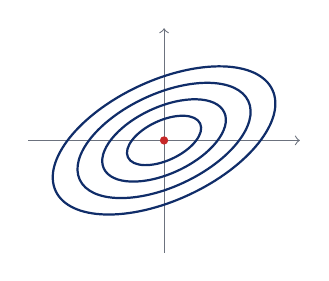
\begin{tikzpicture}[scale=0.75]
        \draw[->,hsegray] (-2.3,0)--(2.3,0); \draw[->,hsegray] (0,-1.9)--(0,1.9);
        \foreach \r in {0.45,0.75,1.05,1.35}{\draw[hseblue,thick,rotate=25] (0,0) ellipse ({1.5*\r} and {0.75*\r});}
        \fill[hseaccent] (0,0) circle (2pt);
      \end{tikzpicture}\\[0.2em]
      {\scriptsize Closed elliptic level sets}
    \end{column}
    \begin{column}{0.32\textwidth}\centering
      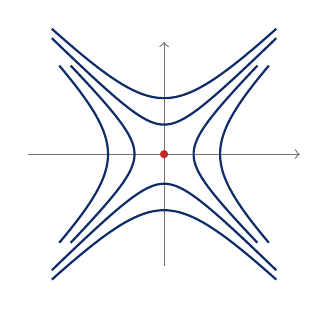
\begin{tikzpicture}[scale=0.75]
        \draw[->,hsegray] (-2.3,0)--(2.3,0); \draw[->,hsegray] (0,-1.9)--(0,1.9);
        \foreach \c in {0.25,0.9}{
            \draw[hseblue,thick,domain=-1.5:1.5,samples=50] plot ({sqrt(\x*\x+\c)},{\x});
            \draw[hseblue,thick,domain=-1.5:1.5,samples=50] plot ({-sqrt(\x*\x+\c)},{\x});
            \draw[hseblue,thick,domain=-1.9:1.9,samples=50] plot ({\x},{sqrt(\x*\x+\c)});
            \draw[hseblue,thick,domain=-1.9:1.9,samples=50] plot ({\x},{-sqrt(\x*\x+\c)});}
        \fill[hseaccent] (0,0) circle (2pt);
      \end{tikzpicture}\\[0.2em]
      {\scriptsize Hyperbolic level sets}
    \end{column}
    \begin{column}{0.32\textwidth}\centering
      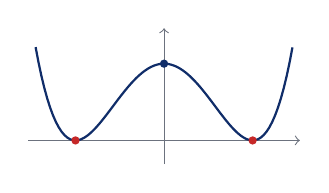
\begin{tikzpicture}[scale=0.75]
        \draw[->,hsegray] (-2.3,0)--(2.3,0); \draw[->,hsegray] (0,-0.4)--(0,1.9);
        \draw[hseblue,thick,domain=-1.45:1.45,samples=90] plot ({1.5*\x},{1.3*(\x*\x-1)*(\x*\x-1)});
        \fill[hseaccent] (-1.5,0) circle (2pt); \fill[hseaccent] (1.5,0) circle (2pt);
        \fill[hseblue] (0,1.3) circle (2pt);
      \end{tikzpicture}\\[0.2em]
      {\scriptsize A one-dimensional slice}
    \end{column}
  \end{columns}
  \vspace{0.7em}
  \takeaway{question}{Which of the three marked points are local minima, which are global, and which piece of
    information --- the gradient or the Hessian --- did you actually use to decide?}
\end{frame}

% ===================================================================
\begin{frame}{Local and global minima: the definitions we will use all year}
  {The only difference is the size of the neighbourhood.}
  \vspace{0.3em}
  Let $f:\mathbb{R}^n\to\mathbb{R}$ be defined on a region $\Omega\subset\mathbb{R}^n$.
  \vspace{0.5em}
  \begin{columns}[T,onlytextwidth]
    \begin{column}{0.5\textwidth}
      \kicker{local minimum}\\[0.3em]
      $x^\ast\in\Omega$ is a local minimum if there exists $\varepsilon>0$ such that
      \[ f(x)\ \ge\ f(x^\ast)\quad\text{for all } x\in\Omega\setminus\{x^\ast\},\ \|x-x^\ast\|<\varepsilon. \]
    \end{column}
    \begin{column}{0.5\textwidth}
      \kicker{global minimum}\\[0.3em]
      $x^\ast\in\Omega$ is a global minimum if
      \[ f(x)\ \ge\ f(x^\ast)\quad\text{for all } x\in\Omega\setminus\{x^\ast\}. \]
    \end{column}
  \end{columns}
  \vspace{0.6em}
  Replacing $\ge$ by $>$ gives the \emph{strict} versions.
  \vspace{0.7em}
  \takeaway{takeaway}{A global minimum is a local minimum whose neighbourhood is the whole of $\Omega$.
    So every global minimum is local --- and the converse fails, which is why the whole course exists.}
\end{frame}

% ===================================================================
\begin{frame}{Gradient and Hessian: notation and shapes}
  {Fix the conventions now; a shape error is a mathematical error.}
  \vspace{0.2em}
  \begin{columns}[T,onlytextwidth]
    \begin{column}{0.52\textwidth}
      \[ \nabla f=\Big(\tfrac{\partial f}{\partial x_1},\ \tfrac{\partial f}{\partial x_2},\ \dots,\
        \tfrac{\partial f}{\partial x_n}\Big)^{\!\top}\in\mathbb{R}^{n} \]
      \[ H(x)=\Big[\tfrac{\partial^2 f}{\partial x_i\,\partial x_j}\Big]_{i,j=1}^{n}\in\mathbb{R}^{n\times n} \]
      \vspace{-0.4em}
      \begin{itemize}\small
        \item $H$ is symmetric whenever the second partials are continuous (Schwarz).
        \item For a quadratic function $H$ is a constant matrix; in general it depends on $x$.
      \end{itemize}
    \end{column}
    \begin{column}{0.45\textwidth}
      \kicker{worked example from the lecture}\\[0.4em]
      $f(x)=3x_1^{3}+2x_1x_2^{2}+4x_2^{2}$ at $x=(1,1)$.
      \[ \tfrac{\partial f}{\partial x_1}=9x_1^{2}+2x_2^{2},\qquad
        \tfrac{\partial f}{\partial x_2}=4x_1x_2+8x_2 \]
      \[ H(x)=\begin{pmatrix} 18x_1 & 4x_2\\ 4x_2 & 4x_1+8\end{pmatrix} \]
      \[ H(1,1)=\begin{pmatrix}18&4\\4&12\end{pmatrix},\quad \det H = 200 \]
    \end{column}
  \end{columns}
\end{frame}

% ===================================================================
\begin{frame}{Block 1 \textperiodcentered\ Exercise 1}{Warm-up on a symmetric quadratic. Three minutes on your own.}
  \vspace{0.6em}
  \kicker{problem}
  \[ f(x_1,x_2)=x_1^{2}+x_2^{2}-x_1x_2 \]
  \vspace{-0.5em}
  \begin{enumerate}\small
    \item Find $\nabla f$ at an arbitrary point.
    \item Find the Hessian $H$.
    \item Evaluate both at $(1,1)$.
    \item Before computing: will $H$ depend on the point? Why?
  \end{enumerate}
  \vspace{0.5em}
  \takeaway{hint}{Write the function as $\tfrac12 x^{\top}Ax$ and read off $A$. Which $A$ do you get,
    and is it the matrix of coefficients you see in the formula?}
\end{frame}

\begin{frame}{Exercise 1 --- solution}{The Hessian of a quadratic is constant; the gradient is not.}
  \vspace{0.3em}
  \[ \nabla f=\begin{pmatrix}2x_1-x_2\\ 2x_2-x_1\end{pmatrix},
    \qquad
    H=\begin{pmatrix}2&-1\\-1&2\end{pmatrix} \]
  \vspace{-0.3em}
  \[ \nabla f(1,1)=\begin{pmatrix}1\\1\end{pmatrix}\neq 0,
    \qquad H(1,1)=\begin{pmatrix}2&-1\\-1&2\end{pmatrix} \]
  \begin{columns}[T,onlytextwidth]
    \begin{column}{0.48\textwidth}
      \kicker{note 1}\\[0.2em]
      {\small $(1,1)$ is \emph{not} stationary: $\nabla f\neq 0$ there, so it cannot be a minimum
        of an unconstrained problem.}
    \end{column}
    \begin{column}{0.48\textwidth}
      \kicker{note 2}\\[0.2em]
      {\small The cross term $-x_1x_2$ contributes $-1$ to \emph{both} off-diagonal entries:
        $f=\tfrac12x^\top Ax$ with $A=H$.}
    \end{column}
  \end{columns}
  \vspace{0.6em}
  \takeaway{takeaway}{Eigenvalues of $H$ are $1$ and $3$: positive definite everywhere, so $f$ is strictly convex
    and its unique minimum is at the origin.}
\end{frame}

% ===================================================================
\begin{frame}{Block 1 \textperiodcentered\ Exercise 2}{Same routine, but now the Hessian moves with the point.}
  \vspace{0.6em}
  \kicker{problem}
  \[ f(x_1,x_2)=3x_1^{3}+2x_1x_2^{2}+4x_2^{2}\qquad\text{at } x=(2,-1) \]
  \vspace{-0.5em}
  \begin{enumerate}\small
    \item Compute $\nabla f(2,-1)$.
    \item Compute $H(2,-1)$ and its determinant.
    \item Compare with the lecture, where the same function was evaluated at $(1,1)$.
    \item Is $(2,-1)$ a stationary point?
  \end{enumerate}
  \vspace{0.5em}
  \takeaway{watch out}{Signs. Two of the four entries change sign when $x_2$ becomes negative.}
\end{frame}

\begin{frame}{Exercise 2 --- solution}{A cubic term makes curvature a local property.}
  \vspace{0.2em}
  \[ \frac{\partial f}{\partial x_1}=9x_1^{2}+2x_2^{2}=9\cdot4+2\cdot1=38,\qquad
    \frac{\partial f}{\partial x_2}=4x_1x_2+8x_2=-8-8=-16 \]
  \[ H(x)=\begin{pmatrix}18x_1 & 4x_2\\ 4x_2 & 4x_1+8\end{pmatrix}
    \;\Rightarrow\;
    H(2,-1)=\begin{pmatrix}36&-4\\-4&16\end{pmatrix},\qquad \det H = 576-16=560 \]
  \vspace{0.2em}
  \begin{columns}[T,onlytextwidth]
    \begin{column}{0.48\textwidth}
      \kicker{answer to (4)}\\[0.2em]
      {\small $\nabla f(2,-1)=(38,-16)^{\top}\neq 0$, so the point is not stationary and the Hessian
        says nothing about optimality here.}
    \end{column}
    \begin{column}{0.48\textwidth}
      \kicker{answer to (3)}\\[0.2em]
      {\small At $(1,1)$ we got $\det H=200$, here $560$. For non-quadratic $f$, curvature is a
        \emph{local} object --- it changes from point to point.}
    \end{column}
  \end{columns}
\end{frame}

% ===================================================================
\begin{frame}{Block 1 \textperiodcentered\ Exercise 3}{Three variables, and our first use of Sylvester's criterion.}
  \vspace{0.6em}
  \kicker{problem}
  \[ f(x_1,x_2,x_3)=x_1^{2}+2x_2^{2}+3x_3^{2}+2x_1x_2-x_2x_3 \]
  \vspace{-0.5em}
  \begin{enumerate}\small
    \item Find $\nabla f$ and $H$.
    \item Decide whether $H$ is positive definite.
    \item What does your answer imply about convexity of $f$ on $\mathbb{R}^3$?
    \item Where is the minimum, and is it unique?
  \end{enumerate}
  \vspace{0.5em}
  \takeaway{hint}{A cross term $c\,x_ix_j$ with $i\neq j$ puts $c$ into \emph{both} entries $H_{ij}$
    and $H_{ji}$ --- the Hessian entry is the second derivative itself. (The matrix $A$ in $f=x^{\top}\!Ax$
    would get $c/2$; do not mix the two conventions.)}
\end{frame}

\begin{frame}{Exercise 3 --- solution}{Leading principal minors decide definiteness without eigenvalues.}
  \vspace{-0.2em}
  \[ \nabla f=\begin{pmatrix}2x_1+2x_2\\ 4x_2+2x_1-x_3\\ 6x_3-x_2\end{pmatrix},
    \qquad
    H=\begin{pmatrix}2&2&0\\2&4&-1\\0&-1&6\end{pmatrix}\ \ \text{(constant)} \]
  \vspace{-0.3em}
  \[ \Delta_1=2>0,\qquad \Delta_2=2\cdot 4-2\cdot 2=4>0,\qquad \Delta_3=\det H=22>0 \]
  \vspace{-0.5em}
  {\footnotesize Expansion along the first row: $\Delta_3=2(4\cdot 6-1)-2(2\cdot 6-0)+0=46-24=22$.}
  \par\vspace{0.9em}
  {\small So $H\succ 0$: the function is strictly convex on $\mathbb{R}^3$, the stationary point
    $\nabla f=0$ is unique and is the global minimum; solving the linear system gives $x^\ast=0$.}
  \vspace{0.4em}
  \takeaway{takeaway}{For a quadratic function, ``strictly convex'' and ``unique global minimum'' are the same
    statement about one constant matrix.}
\end{frame}

% ===================================================================
\begin{frame}{Sylvester's criterion --- and the trap inside it}
  {It answers ``definite or not''. It does not answer ``semidefinite or not''.}
  \vspace{0.1em}
  Let $\Delta_k$ be the $k$-th \emph{leading} principal minor of a symmetric $A$.
  \vspace{0.3em}
  \begin{columns}[T,onlytextwidth]
    \begin{column}{0.47\textwidth}
      \kicker{the criterion}\\[0.3em]
      {\footnotesize
        $A\succ 0 \iff \Delta_k>0$ for all $k$.\\[0.35em]
        $A\prec 0 \iff (-1)^k\Delta_k>0$ for all $k$, i.e.\ signs alternate starting with $-$.\\[0.35em]
        Otherwise: indefinite \emph{or} semidefinite --- the leading minors cannot tell which.}
    \end{column}
    \begin{column}{0.5\textwidth}
      \kicker{counterexample to remember}\\[0.3em]
      \[ A=\begin{pmatrix}0&0\\0&-1\end{pmatrix}:\quad \Delta_1=0,\ \Delta_2=0 \]
      {\small Both leading minors are non-negative, yet $A$ is negative semidefinite. For semidefiniteness
        you must check \emph{all} principal minors, not only the leading ones.}
    \end{column}
  \end{columns}
  \vspace{0.4em}
  \takeaway{practical rule}{On paper use Sylvester for strict definiteness. In code use
    \texttt{numpy.linalg.eigvalsh} with a tolerance --- it is the honest tool for the borderline cases.}
\end{frame}

% ===================================================================
\begin{frame}{Optimality conditions: the summary table}
  {Necessary conditions filter candidates. Only the sufficient condition certifies an answer.}
  \vspace{0.5em}
  \centering
  \begin{tabular}{@{}l l l@{}}
    \toprule
                 & \textbf{Necessary}                    & \textbf{Sufficient}                         \\
    \midrule
    First order  & $\nabla f(x^\ast)=0$ (interior point) & ---                                         \\[0.35em]
    Second order & $H(x^\ast)\succeq 0$                  & $\nabla f(x^\ast)=0$ and $H(x^\ast)\succ 0$ \\
    \bottomrule
  \end{tabular}
  \vspace{0.9em}
  \begin{columns}[T,onlytextwidth]
    \begin{column}{0.48\textwidth}
      \kicker{at the boundary}\\[0.25em]
      {\small The equality weakens to an inequality: $s^{\top}\nabla f(x^\ast)\ge 0$ for every feasible
        direction $s$. That inequality is the seed of KKT theory later in the course.}
    \end{column}
    \begin{column}{0.48\textwidth}
      \kicker{the gap}\\[0.25em]
      {\small Between $\succeq 0$ and $\succ 0$ lives everything interesting: flat directions, where the
        second-order test simply has no opinion. Exercises 6 and 7 live exactly there.}
    \end{column}
  \end{columns}
\end{frame}

% ===================================================================
\begin{frame}{Block 2 \textperiodcentered\ Exercise 4}{The simplest landscape there is. Two minutes.}
  \vspace{0.6em}
  \kicker{problem}
  \[ f(x_1,x_2)=x_1^{2}+x_2^{2} \]
  \vspace{-0.5em}
  \begin{enumerate}\small
    \item Find all stationary points.
    \item Compute the Hessian and decide its definiteness.
    \item Which of the two conditions --- necessary or sufficient --- did you just use?
    \item Is the point a \emph{global} minimum, and what exactly justifies that?
  \end{enumerate}
  \vspace{0.5em}
  \takeaway{watch the wording}{``The Hessian is positive definite'' certifies a \emph{local} minimum.
    Global needs one extra sentence --- find it.}
\end{frame}

% ===================================================================
\begin{frame}{Exercise 4 --- solution}{A bowl: positive curvature in every direction.}
  \vspace{0.2em}
  \begin{columns}[T,onlytextwidth]
    \begin{column}{0.42\textwidth}\centering
      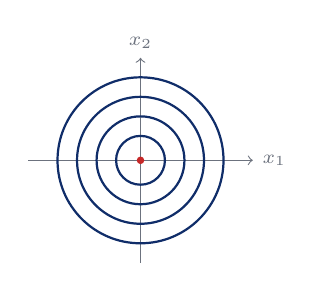
\begin{tikzpicture}[scale=0.62]
        \draw[->,hsegray] (-2.3,0)--(2.3,0) node[right,font=\scriptsize]{$x_1$};
        \draw[->,hsegray] (0,-2.1)--(0,2.1) node[above,font=\scriptsize]{$x_2$};
        \foreach \r in {0.5,0.9,1.3,1.7}{\draw[hseblue,thick] (0,0) circle (\r);}
        \fill[hseaccent] (0,0) circle (2.2pt);
      \end{tikzpicture}\\[0.2em]
      {\scriptsize Level sets are circles}
    \end{column}
    \begin{column}{0.54\textwidth}
      \[ \nabla f=\begin{pmatrix}2x_1\\2x_2\end{pmatrix}=0\ \Rightarrow\ x^\ast=(0,0) \]
      \[ H=\begin{pmatrix}2&0\\0&2\end{pmatrix},\qquad \Delta_1=2>0,\ \ \Delta_2=4>0 \]
      {\small $H\succ0$, so the sufficient condition applies: $(0,0)$ is a \emph{strict local} minimum.
        Global follows separately --- either from convexity ($H\succeq0$ everywhere) or directly from
        $f(x)=x_1^2+x_2^2\ge0=f(0,0)$.}
    \end{column}
  \end{columns}
  \vspace{0.4em}
  \takeaway{takeaway}{Eigenvalues $2$ and $2$: the same curvature in every direction, which is why the level
    sets are perfect circles and why gradient descent would land here in a single step.}
\end{frame}

% ===================================================================
\begin{frame}{Block 2 \textperiodcentered\ Exercise 5}{Same gradient structure, opposite conclusion. Two minutes.}
  \vspace{0.6em}
  \kicker{problem}
  \[ f(x_1,x_2)=x_1^{2}-x_2^{2} \]
  \vspace{-0.5em}
  \begin{enumerate}\small
    \item Show that $(0,0)$ is a stationary point.
    \item Show that it is neither a minimum nor a maximum.
    \item Do it \emph{without} drawing a picture --- a picture is a guide, not a proof.
  \end{enumerate}
  \vspace{0.5em}
  \takeaway{hint}{Restrict the function to a line through the origin. Two well-chosen lines settle the question
    completely.}
\end{frame}

% ===================================================================
\begin{frame}{Exercise 5 --- solution}{Mixed curvature signs always mean a saddle.}
  \vspace{0.2em}
  \begin{columns}[T,onlytextwidth]
    \begin{column}{0.42\textwidth}\centering
      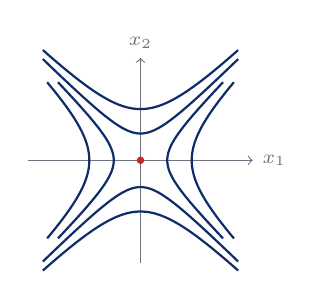
\begin{tikzpicture}[scale=0.62]
        \draw[->,hsegray] (-2.3,0)--(2.3,0) node[right,font=\scriptsize]{$x_1$};
        \draw[->,hsegray] (0,-2.1)--(0,2.1) node[above,font=\scriptsize]{$x_2$};
        \foreach \c in {0.3,1.1}{
            \draw[hseblue,thick,domain=-1.6:1.6,samples=50] plot ({sqrt(\x*\x+\c)},{\x});
            \draw[hseblue,thick,domain=-1.6:1.6,samples=50] plot ({-sqrt(\x*\x+\c)},{\x});
            \draw[hseblue,thick,domain=-2:2,samples=50] plot ({\x},{sqrt(\x*\x+\c)});
            \draw[hseblue,thick,domain=-2:2,samples=50] plot ({\x},{-sqrt(\x*\x+\c)});}
        \fill[hseaccent] (0,0) circle (2.2pt);
      \end{tikzpicture}\\[0.2em]
      {\scriptsize Level sets are hyperbolas}
    \end{column}
    \begin{column}{0.54\textwidth}
      \[ \nabla f=\begin{pmatrix}2x_1\\-2x_2\end{pmatrix}=0\ \Rightarrow\ (0,0) \]
      \[ H=\begin{pmatrix}2&0\\0&-2\end{pmatrix},\qquad \Delta_1=2>0,\ \ \Delta_2=-4<0 \]
      {\footnotesize Neither Sylvester pattern holds: the matrix is indefinite, with eigenvalues $2$ and $-2$.
        The proof without pictures: $f(x_1,0)=x_1^{2}>0$ and $f(0,x_2)=-x_2^{2}<0$, so every neighbourhood of the
        origin contains larger \emph{and} smaller values.}
    \end{column}
  \end{columns}
  \vspace{0.3em}
  \takeaway{takeaway}{The gradient locates candidates; the eigenvalue \emph{signs} classify them.
    Mixed signs always mean a saddle.}
\end{frame}

% ===================================================================
\begin{frame}{Block 2 \textperiodcentered\ Exercise 6: the monkey saddle}{Where the second-order test runs out of information.}
  \vspace{0.5em}
  \kicker{problem}
  \[ f(x_1,x_2)=x_1^{3}-3x_1x_2^{2} \]
  \vspace{-0.4em}
  \begin{enumerate}\small
    \item Find all stationary points.
    \item Write the Hessian and evaluate it at the origin.
    \item Try to classify the point with the tools from the table. What happens?
    \item Find a direction that settles the question.
  \end{enumerate}
  \vspace{0.5em}
  \takeaway{hint}{When the Hessian is the zero matrix, stop using theorems and start using the
    \emph{definition}: compare $f$ with $f(x^\ast)$ along a cleverly chosen line.}
\end{frame}

\begin{frame}{Exercise 6 --- solution}{The name comes from the three valleys: two for the legs, one for the tail.}
  \vspace{0.1em}
  \begin{columns}[T,onlytextwidth]
    \begin{column}{0.58\textwidth}
      {\small
        \[ \frac{\partial f}{\partial x_1}=3x_1^{2}-3x_2^{2},\quad
          \frac{\partial f}{\partial x_2}=-6x_1x_2 \]
        From the second equation $x_1=0$ or $x_2=0$; the first one then leaves only $(0,0)$.
        \[ H(x)=\begin{pmatrix}6x_1&-6x_2\\-6x_2&-6x_1\end{pmatrix}
          \;\Rightarrow\; H(0,0)=\begin{pmatrix}0&0\\0&0\end{pmatrix} \]
        The zero matrix is both $\succeq 0$ and $\preceq 0$: the necessary condition holds trivially, the
        sufficient one does not apply, and all $\Delta_k=0$, so Sylvester is silent.
        Along $x_2=0$ we get $f(x_1,0)=x_1^{3}$, which changes sign at the origin: the point is
        neither a minimum nor a maximum.}
    \end{column}
    \begin{column}{0.38\textwidth}\centering
      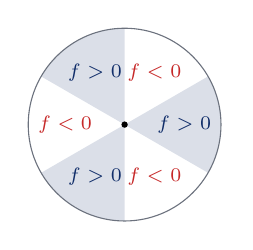
\begin{tikzpicture}[scale=0.72]
        \foreach \a in {0,120,240}{
            \fill[hseblue!15] (0,0) -- (\a-30:1.7) arc (\a-30:\a+30:1.7) -- cycle;}
        \draw[hsegray] (0,0) circle (1.7);
        \foreach \a in {0,120,240}{\node[hseblue,font=\scriptsize] at (\a:1.05) {$f>0$};}
        \foreach \a in {60,180,300}{\node[hseaccent,font=\scriptsize] at (\a:1.05) {$f<0$};}
        \fill (0,0) circle (1.6pt);
      \end{tikzpicture}\\[0.4em]
      {\scriptsize Six alternating sectors around the origin}
    \end{column}
  \end{columns}
\end{frame}

% ===================================================================
\begin{frame}{Block 2 \textperiodcentered\ Exercise 7}{One more zero Hessian --- and this time the answer is different. Two minutes.}
  \vspace{0.6em}
  \kicker{problem}
  \[ f(x_1,x_2)=x_1^{4}+x_2^{4} \]
  \vspace{-0.5em}
  \begin{enumerate}\small
    \item Find the stationary points and the Hessian at the origin.
    \item Try the second-order test. What does it say?
    \item Decide the question anyway --- in one line.
    \item Compare your answer with Exercise 6. What is different, and what is identical?
  \end{enumerate}
  \vspace{0.5em}
  \takeaway{hint}{You do not need any theorem here. Look at the sign of the function itself.}
\end{frame}

% ===================================================================
\begin{frame}{Exercise 7 --- solution}{Identical first- and second-order data, opposite answers.}
  \vspace{0.2em}
  \[ \nabla f=(4x_1^{3},4x_2^{3})^{\top}=0\ \Rightarrow\ (0,0),\qquad
    H(x)=\begin{pmatrix}12x_1^{2}&0\\0&12x_2^{2}\end{pmatrix}\ \Rightarrow\
    H(0,0)=\begin{pmatrix}0&0\\0&0\end{pmatrix} \]
  {\small Direct argument: $f(x)=x_1^{4}+x_2^{4}\ge 0=f(0,0)$, with equality only at the origin, so the origin
    is a \emph{strict global} minimum --- no theorem required.}
  \par\medskip
  \begin{center}\small
    \begin{tabular}{@{}l c c l@{}}
      \toprule
      \textbf{Function}     & $\nabla f(0)$ & $H(0)$ & \textbf{Truth}              \\
      \midrule
      $x_1^{4}+x_2^{4}$     & $0$           & $0$    & strict global minimum       \\
      $x_1^{3}-3x_1x_2^{2}$ & $0$           & $0$    & neither minimum nor maximum \\
      \bottomrule
    \end{tabular}
  \end{center}
  \takeaway{takeaway}{Same data, opposite answers. When the Hessian is singular, the second-order test is not
    ``inconclusive by bad luck'' --- it provably cannot decide.}
\end{frame}

% ===================================================================
\begin{frame}{Block 3 \textperiodcentered\ Convexity: definitions}
  {The property that turns a local statement into a global one.}
  \vspace{0.4em}
  \begin{columns}[T,onlytextwidth]
    \begin{column}{0.48\textwidth}
      \kicker{convex set}\\[0.3em]
      {\small $\Omega$ is convex if for any $x_1,x_2\in\Omega$ the whole segment $[x_1,x_2]$ lies in $\Omega$:}
      \[ \lambda x_1+(1-\lambda)x_2\in\Omega,\quad \lambda\in[0,1] \]
    \end{column}
    \begin{column}{0.48\textwidth}
      \kicker{convex function}\\[0.3em]
      {\small $f$ is convex on a convex $\Omega$ if for all $x,y\in\Omega$, $\lambda\in[0,1]$:}
      \[ f(\lambda x+(1-\lambda)y)\le \lambda f(x)+(1-\lambda)f(y) \]
    \end{column}
  \end{columns}
  \vspace{0.6em}
  {\small Geometrically: the graph never rises above the chord connecting two of its points.
    For $f\in C^2$ this is equivalent to $H(x)\succeq 0$ for every $x\in\Omega$.}
  \vspace{0.6em}
  \takeaway{why we care}{For a convex $f$ on a convex $\Omega$, every local minimum is global, and
    $\nabla f(x^\ast)=0$ stops being merely necessary --- it becomes sufficient.}
\end{frame}

\begin{frame}{Block 3 \textperiodcentered\ Exercise 8}{A proof straight from the definition. Two minutes.}
  \vspace{0.6em}
  \kicker{problem}
  \[ \Omega=\{(x_1,x_2):\ x_1^{2}+x_2^{2}\le 4\} \]
  \vspace{-0.5em}
  \begin{enumerate}\small
    \item Prove from the definition that $\Omega$ is convex.
    \item Which properties of the norm did your proof use?
    \item Does the same argument work for a square? For a ring?
  \end{enumerate}
  \vspace{0.5em}
  \takeaway{hint}{Rewrite the set as $\{x:\|x\|\le2\}$. Then take $z=\lambda x+(1-\lambda)y$ and estimate
    $\|z\|$ --- two standard inequalities are enough.}
\end{frame}

% ===================================================================
\begin{frame}{Exercise 8 --- solution}{Convexity of any ball is the triangle inequality in disguise.}
  \vspace{0.4em}
  Take $x,y\in\Omega$, so $\|x\|\le2$ and $\|y\|\le2$, and take $\lambda\in[0,1]$. Put
  $z=\lambda x+(1-\lambda)y$. Then
  \[ \|z\|=\|\lambda x+(1-\lambda)y\|
    \ \overset{(1)}{\le}\ \|\lambda x\|+\|(1-\lambda)y\|
    \ \overset{(2)}{=}\ \lambda\|x\|+(1-\lambda)\|y\|
    \ \le\ 2\lambda+2(1-\lambda)=2, \]
  where $(1)$ is the triangle inequality and $(2)$ is homogeneity of the norm (the factors are non-negative,
  so no absolute values are needed). Hence $z\in\Omega$, and $\Omega$ is convex. $\blacksquare$
  \vspace{0.5em}
  \takeaway{how far it generalises}{Nothing but two norm properties was used, so \emph{every} ball in
    \emph{every} norm is convex --- including the $\ell_1$ diamond and the $\ell_\infty$ square, which have
    corners. A ring is not convex: the segment between two opposite points crosses the hole.}
\end{frame}

% ===================================================================
\begin{frame}{Block 3 \textperiodcentered\ Exercise 9}{Convexity of a quadratic, decided by one matrix. Two minutes.}
  \vspace{0.6em}
  \kicker{problem}
  \[ f(x_1,x_2)=x_1^{2}+x_2^{2}-4x_1x_2 \]
  \vspace{-0.5em}
  \begin{enumerate}\small
    \item Is $f$ convex on $\mathbb{R}^2$?
    \item Compare with Exercise 1, where the cross term was $-x_1x_2$. What changed?
    \item For which $a$ is $x_1^{2}+x_2^{2}+a\,x_1x_2$ convex?
  \end{enumerate}
  \vspace{0.5em}
  \takeaway{hint}{For a quadratic the Hessian is constant, so convexity is a single yes/no question about a
    single matrix.}
\end{frame}

% ===================================================================
\begin{frame}{Exercise 9 --- solution}{It is not the sign of the cross term that matters --- it is its size.}
  \vspace{0.3em}
  \[ H=\begin{pmatrix}2&-4\\-4&2\end{pmatrix}\ \text{(constant)},\qquad
    \Delta_1=2>0,\qquad \Delta_2=4-16=-12<0 \]
  {\small Neither Sylvester pattern holds, so $H$ is indefinite --- eigenvalues $6$ and $-2$. Since $H$ is the
    same at every point, it is nowhere $\succeq0$, and therefore $f$ is \emph{not} convex on $\mathbb{R}^2$.}
  \par\medskip
  For the whole family $f_a=x_1^{2}+x_2^{2}+a\,x_1x_2$ the Hessian is
  $\left(\begin{smallmatrix}2&a\\a&2\end{smallmatrix}\right)$ with eigenvalues $2\pm a$:
  \[ \text{convex}\iff|a|\le2,\qquad \text{strictly convex}\iff|a|<2. \]
  \takeaway{takeaway}{Exercise 1 had $a=-1$ (eigenvalues $1,3$, convex); here $a=-4$ (eigenvalues $-2,6$, not
    convex). The cross term competes with the squares, and at $|a|=2$ it exactly ties: $f=(x_1\pm x_2)^2$ has a
    whole line of minima.}
\end{frame}

% ===================================================================
\begin{frame}{Block 4 \textperiodcentered\ Feasible directions and directional derivatives}
  {What optimality means when you are standing on the boundary.}
  \vspace{0.2em}
  \begin{columns}[T,onlytextwidth]
    \begin{column}{0.62\textwidth}
      {\small
        \kicker{feasible direction}\par\smallskip
        $s\neq 0$ is feasible at $x\in\Omega$ if there is $\alpha_0>0$ with
        $x+\alpha s\in\Omega$ for all $\alpha\in[0,\alpha_0]$.
        \par\medskip
        \kicker{directional derivative}
        \[ \frac{\partial f}{\partial s}(x)=\lim_{\alpha\to 0}\frac{f(x+\alpha s)-f(x)}{\alpha}
          = s^{\top}\nabla f(x) \]
        If $\|s\|=1$ this is the rate of increase of $f$ along $s$.
        \par\smallskip
        \kicker{first-order necessary condition}
        \[ s^{\top}\nabla f(x^\ast)\ \ge\ 0\quad\text{for every feasible } s \]
        Interior point: every direction is feasible, so $\pm s$ both qualify and this collapses to
        $\nabla f(x^\ast)=0$.}
    \end{column}
    \begin{column}{0.36\textwidth}\centering
      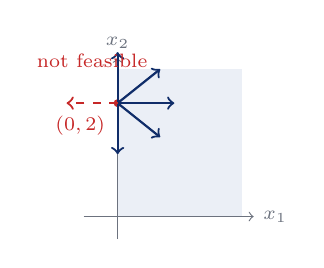
\begin{tikzpicture}[scale=0.72]
        \fill[hselight] (0,0) rectangle (2.2,2.6);
        \draw[->,hsegray] (-0.6,0)--(2.4,0) node[right,font=\scriptsize]{$x_1$};
        \draw[->,hsegray] (0,-0.4)--(0,2.8) node[above,font=\scriptsize]{$x_2$};
        \fill[hseaccent] (0,2) circle (2pt);
        \node[hseaccent,font=\scriptsize,below left=1pt] at (0,2) {$(0,2)$};
        \draw[->,hseblue,thick] (0,2)--(1.0,2);
        \draw[->,hseblue,thick] (0,2)--(0.75,2.6);
        \draw[->,hseblue,thick] (0,2)--(0.75,1.4);
        \draw[->,hseblue,thick] (0,2)--(0,2.9);
        \draw[->,hseblue,thick] (0,2)--(0,1.1);
        \draw[->,hseaccent,dashed,thick] (0,2)--(-0.9,2);
        \node[hseaccent,font=\scriptsize] at (-0.45,2.75) {not feasible};
      \end{tikzpicture}\\[0.4em]
      {\scriptsize Feasible cone at $(0,2)$ in the first quadrant}
    \end{column}
  \end{columns}
\end{frame}

\begin{frame}{Block 4 \textperiodcentered\ Exercise 10}{Optimality on the boundary. Three minutes.}
  \vspace{0.6em}
  \kicker{problem}
  \[ \Omega=\{x_1\ge0,\ x_2\ge0\},\qquad x=(0,2),\qquad f(x_1,x_2)=x_1+x_2 \]
  \vspace{-0.5em}
  \begin{enumerate}\small
    \item Which constraints are active at $(0,2)$?
    \item Describe the full set of feasible directions there.
    \item Check the first-order necessary condition $s^{\top}\nabla f\ge0$.
    \item If it fails, produce the direction that breaks it.
  \end{enumerate}
  \vspace{0.5em}
  \takeaway{hint}{One coordinate is pinned at its bound, the other has room on both sides. That asymmetry is
    the whole exercise.}
\end{frame}

% ===================================================================
\begin{frame}{Exercise 10 --- solution}{One bad direction is enough to disqualify a point.}
  \vspace{0.2em}
  $\Omega=\{x_1\ge 0,\ x_2\ge 0\}$, the point $x=(0,2)$, the objective $f(x_1,x_2)=x_1+x_2$.
  \vspace{0.5em}
  \begin{itemize}\small
    \item $x_1=0$ is active, $x_2=2>0$ is not. Hence the feasible set of directions is
          \[ \{s=(s_1,s_2)\neq 0:\ s_1\ge 0,\ s_2\in\mathbb{R}\}. \]
    \item $\nabla f\equiv(1,1)^{\top}$, so the condition to test is $s^{\top}\nabla f=s_1+s_2\ge 0$
          for \emph{every} feasible $s$.
    \item Take $s=(0,-1)$: feasible, and $s^{\top}\nabla f=-1<0$.
  \end{itemize}
  \vspace{0.4em}
  Therefore $(0,2)$ fails the first-order necessary condition and is not a candidate for a local minimum ---
  consistent with the true minimiser $(0,0)$.
  \vspace{0.5em}
  \takeaway{takeaway}{To \emph{reject} a point you need one violating direction. To \emph{accept} it you must
    check all of them --- which is precisely why we will later replace this test by KKT multipliers.}
\end{frame}

\begin{frame}{Block 4 \textperiodcentered\ Exercise 11}{Definition versus formula. Three minutes.}
  \vspace{0.6em}
  \kicker{problem}
  \[ f(x_1,x_2)=x_1^{2}+2x_2^{2},\qquad x=(1,1),\qquad s=(1,-1) \]
  \vspace{-0.5em}
  \begin{enumerate}\small
    \item Compute $\dfrac{\partial f}{\partial s}(x)$ from the definition, through the limit.
    \item Compute it again as $s^{\top}\nabla f(x)$.
    \item Is $s$ a descent direction?
    \item Careful: is your number a rate per unit of $\alpha$, or per unit of length?
  \end{enumerate}
  \vspace{0.5em}
  \takeaway{hint}{For part 1 substitute $x+\alpha s$ into $f$, expand, and let $\alpha\to0$. You should get a
    quadratic in $\alpha$ whose constant term is $f(x)$.}
\end{frame}

% ===================================================================
\begin{frame}{Exercise 11 --- solution}{The formula and the definition must agree; verifying that is the point.}
  $f(x_1,x_2)=x_1^{2}+2x_2^{2}$ at $x=(1,1)$ along $s=(1,-1)$.
  \par\medskip
  \begin{columns}[T,onlytextwidth]
    \begin{column}{0.52\textwidth}
      \kicker{way 1: from the definition}
      \begin{align*}
        f(x+\alpha s) & =(1+\alpha)^2+2(1-\alpha)^2 \\
                      & =3-2\alpha+3\alpha^{2}
      \end{align*}
      \[ \frac{\partial f}{\partial s}=\lim_{\alpha\to0}\frac{(3-2\alpha+3\alpha^{2})-3}{\alpha}=-2 \]
    \end{column}
    \begin{column}{0.45\textwidth}
      \kicker{way 2: from the gradient}
      \[ \nabla f=(2x_1,4x_2)^{\top}\ \Rightarrow\ \nabla f(1,1)=(2,4)^{\top} \]
      \[ s^{\top}\nabla f = 1\cdot 2+(-1)\cdot 4=-2 \]
      {\small Both routes give $-2$, so $(1,-1)$ is a descent direction at $(1,1)$.}
    \end{column}
  \end{columns}
  \par\medskip
  \takeaway{note on normalisation}{$\|s\|=\sqrt2\neq 1$, so $-2$ is a rate per unit of $\alpha$, not per unit
    of length: per unit length it is $-2/\sqrt2=-\sqrt2$.}
\end{frame}

% ===================================================================
\begin{frame}[fragile]{From the board to the keyboard}
  {Every statement of today has a three-line numerical counterpart. Use them in the homework.}
  \vspace{0.3em}
  \begin{columns}[T,onlytextwidth]
    \begin{column}{0.52\textwidth}
      \begin{lstlisting}
import numpy as np

def central_diff(f, x, h=1e-5):
    x = np.asarray(x, float)
    g = np.empty_like(x)
    for j in range(x.size):
        e = np.zeros_like(x); e[j] = h
        g[j] = (f(x + e) - f(x - e)) / (2*h)
    return g
\end{lstlisting}
    \end{column}
    \begin{column}{0.45\textwidth}
      \begin{lstlisting}
def classify(H, tol=1e-8):
    w = np.linalg.eigvalsh(0.5*(H + H.T))
    if np.all(w > tol):   return "min"
    if np.all(w < -tol):  return "max"
    if w.min() < -tol < w.max():
        return "saddle"
    return "inconclusive"
\end{lstlisting}
    \end{column}
  \end{columns}
  \vspace{0.4em}
  \takeaway{question}{Run \texttt{classify} on the Hessians of $x_1^4+x_2^4$ and $x_1^3-3x_1x_2^2$ at the origin.
    Both return \texttt{"inconclusive"}. Which of the two answers is a limitation of the code, and which is a
    limitation of the mathematics?}
\end{frame}

% ===================================================================
\begin{frame}{Summary}{Five sentences to carry into the next lecture.}
  \vspace{0.5em}
  \begin{enumerate}\small\setlength{\itemsep}{0.4em}
    \item A global minimum is a local minimum with the largest possible neighbourhood; the whole difficulty of
          optimization lives in the gap between the two.
    \item The gradient supplies candidates, the Hessian classifies them --- and only for interior points of $\Omega$.
    \item Necessary conditions cannot certify a minimum; only $\nabla f=0$ together with $H\succ 0$ can.
    \item When $H$ is singular the second-order test is genuinely undecided: $x_1^4+x_2^4$ and $x_1^3-3x_1x_2^2$
          are indistinguishable to it, yet one is a minimum and the other is not.
    \item On the boundary the equality $\nabla f=0$ becomes the inequality $s^{\top}\nabla f\ge 0$ over feasible
          directions --- the starting point of constrained optimization.
  \end{enumerate}
\end{frame}

% ===================================================================
\begin{frame}{Exit ticket and home practice}{Two minutes of writing now; four exercises before the next seminar.}
  \vspace{0.3em}
  \begin{columns}[T,onlytextwidth]
    \begin{column}{0.47\textwidth}
      \kicker{exit ticket (answer in one line each)}\\[0.4em]
      {\small
        \num{1} Give a function whose Hessian is positive semidefinite at a point that is not a local minimum.\\[0.4em]
        \num{2} Why does the first-order condition become an inequality at the boundary?\\[0.4em]
        \num{3} A colleague reports $\Delta_1>0$ and $\Delta_2=0$. What can you conclude?}
    \end{column}
    \begin{column}{0.47\textwidth}
      \kicker{home practice}\\[0.4em]
      {\small
        \num{1} Classify the stationary points of $f=x_1^3+x_2^2$.\\[0.4em]
        \num{2} For which $a$ is $x_1^2+x_2^2+a\,x_1x_2$ convex on $\mathbb{R}^2$?\\[0.4em]
        \num{3} Describe the feasible directions at $(0,0)$ for $\Omega=\{x_1\ge0,\ x_2\ge0\}$.\\[0.4em]
        \num{4} Implement \texttt{classify} and test it on all functions from today; report where it says
        \texttt{"inconclusive"}.}
    \end{column}
  \end{columns}
  \vspace{0.4em}
  \takeaway{next time}{We start descending: how to move from a point that is not optimal to one that is,
    and how fast that is possible.}
\end{frame}

\end{document}
